\scanpage{112}

Carte régulière (orientée)\\
du polygône régulier $P_n$ $(n\geq2)$

en le trouant en les sommets et les centres des faces \uline{et} les milieux des segments

\[
\Sigma_n^{\substack{*\\*}*}
=\Sigma_n\setminus\bigl(S(\Sigma_{\unsure{n}})\cup A(\Sigma_{\unsure{n}})\cup F(\Sigma_n)\bigr)
\]
\margin{sommets}
\margin{centres faces}
\margin{milieux arêtes}

\unsure{diviser} par $D_n^+\subset D_{2n}^+$

\diagram{\begin{tikzcd}[ampersand replacement=\&,column sep=large,row sep=small]
\Sigma_n^{\substack{*\\*}*}
 \arrow[r,"\deg n"] \arrow[dddd,phantom,"\simeq" description]
 \& \Sigma_1^{\substack{*\\*}*}=\mathbb{P}_1\setminus\{\underbrace{0,\infty}_{\text{``pôles''}},1,-1\}
 \arrow[r,"\deg2"]
 \& \Sigma_3^{\substack{*\\\cdot}\cdot}=U_{0\,3} \\
 \& \Vert \& \\
 \& \Sigma_n^{\substack{*\\*}*}/D_n \& \\
 \& \Vert \& \\
\Sigma_{2n}^{\substack{*\\*}\unsure{\cdot}}
 \arrow[r]
 \& \Sigma_2^{\substack{*\\*}\cdot}\arrow[r,"2"]
 \& \Sigma_1^{\substack{*\\*}\cdot}\simeq U_0^3
\end{tikzcd}}

\margin{division \deleted{\unsure{par le}} par $D_n/D_n^+$}
\margin{(carte régulière $\overline{\Sigma}_{\unsure{a|n}}$ \unsure{à deux sommets|à deux arêtes})}

division par $D_{2n}^+$

\margin{%
\figure{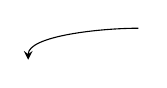
\begin{tikzpicture}[>=stealth]\draw[->] (1.4,0.4) .. controls (0.9,0.4) and (0,0.3) .. (0,0);\end{tikzpicture}}
(on n'a enlevé que les sommets et centres faces)

À cause de cet isomorphisme, on fait \deleted{$\unsure{D_n}$} $D_{2n}$ opérer sur
$\Sigma_n^{\substack{*\\*}*}(\simeq\Sigma_{2n}^{\substack{*\\*}\cdot})$, on peut

donc
}

\diagram{\begin{tikzcd}[ampersand replacement=\&,column sep=large,row sep=large]
 \& \begin{gathered}\Sigma_n^{\substack{*\\*}*}\\\simeq\Sigma_{2n}^{\substack{*\\*}\cdot}\end{gathered}
 \arrow[dl]\arrow[dr] \& \\
\Sigma_{2n}^{\substack{*\\*}\cdot}/D_{2n}^+\arrow[dd]
 \& \& \Sigma_n^{\substack{*\\*}*}/D_n^+\arrow[ll]\arrow[dl] \\
 \& \Sigma^{\substack{*\\*}*}/D_n\arrow[dl,bend left=12] \& \\
\Sigma_{2n}^{\substack{*\\*}\cdot}/D_{2n} \& \&
\end{tikzcd}}

\figure{\begin{tikzpicture}[>=stealth]\draw[->] (0,0) .. controls (0.8,0) and (1.4,0.2) .. (1.6,0.8);\end{tikzpicture}}

\diagram{\begin{tikzpicture}\node (d) at (0,0) {\begin{tikzcd}[ampersand replacement=\&,column sep=large,row sep=large]
 \& \Sigma_n^{\substack{*\\*}*}\simeq\Sigma_{2n}^{\substack{*\\*}\cdot}\arrow[d] \& \\
 \& \Sigma_n^{\substack{*\\*}*}/D_n^+\simeq\Sigma_1^{\substack{\unsure{*}\\*}*}\simeq\Sigma_2^{\substack{*\\*}\cdot}\arrow[dl]\arrow[dr] \& \\
\Sigma^{\substack{*\\*}*}/D_{2n}^+\arrow[dr] \& \& \Sigma_n^{\substack{*\\*}*}/D_n\arrow[dl,dash] \\
 \& \Sigma_n^{\substack{*\\*}\cdot}/D_{2n} \&
\end{tikzcd}};\draw[rounded corners=22pt] (d.south west) rectangle (d.north east);\end{tikzpicture}}

\diagram{\begin{tikzcd}[ampersand replacement=\&]
\Sigma_n^{\substack{*\\*}\cdot}\arrow[r,"D_n^+"] \& \Sigma_1^{\substack{*\\*}\cdot}\simeq U_0^3
\end{tikzcd}}

Si on divise par $D_n$ \deleted{tout} entier, on trouve des ramifications sur les arêtes

\mspage{111}
